%%%%%%%%%%%%%%%%%%%% PREAMBLE %%%%%%%%%%%%%%%%%%%%%%
\documentclass[12pt]{extarticle}
\usepackage[table,xcdraw,dvipsnames]{xcolor}
\colorlet{gold}{green!10!orange!90!}
\usepackage{graphicx}
\usepackage{color}
\usepackage{mathptmx}
\usepackage{gensymb}
\usepackage{amsmath}
\usepackage{placeins}
\usepackage{array}
\usepackage{float}
\usepackage{setspace}
\usepackage[top=1in, bottom=1in, left=1in, right=1in]{geometry}
\usepackage{fancyhdr}
\usepackage{enumerate}
\newcommand{\HRule}{\rule{\linewidth}{0.5mm}}
\setlength{\headheight}{15.2pt}
\pagestyle{fancy}
\usepackage{changepage}
\newenvironment{sect}
  {\adjustwidth{-2.25em}{0pt}}
  {\endadjustwidth}
\newenvironment{subsubs}
  {\adjustwidth{2.25em}{0pt}}
  {\endadjustwidth}
\setlength\extrarowheight{5pt}
\newcolumntype{L}{>{\centering\arraybackslash}m{3cm}}
\usepackage{hyperref} 
\hypersetup{%
  colorlinks=true,% hyperlinks will be coloured
  linkcolor=gray,% hyperlink text will be green
}

\usepackage{geometry}
\usepackage{amsfonts}
\usepackage{xcolor}
\usepackage{listings}
\geometry{a4paper,margin=1in}

\definecolor{green}{rgb}{0,1,0}

\definecolor{purple}{rgb}{0.5,0,0.5}

\definecolor{blue}{rgb}{0,0,1}

\definecolor{orange}{rgb}{1,.6,0}




%%%%%%%%%%%%%%%%%%%% CUSTOM HEADINGS %%%%%%%%%%%%%%%%%%%%%%
%\pagestyle{myheadings}
\lhead{\small{Final Report}}
\chead{\small{Furuta Pendulum}}
\rhead{\small{ASEN 5115}}

\begin{document}
%%%%%%%%%%%%%%%%%%%% TITLE PAGE %%%%%%%%%%%%%%%%%%%%%%
	\begin{titlepage}
		\begin{center}
			% Upper part of the page
			\textsc{\LARGE Un\underline{iversity of Colorado at Bould}er}\\[0.5cm]
			\textsc{\Large Master's Project}\\[1.5cm]
			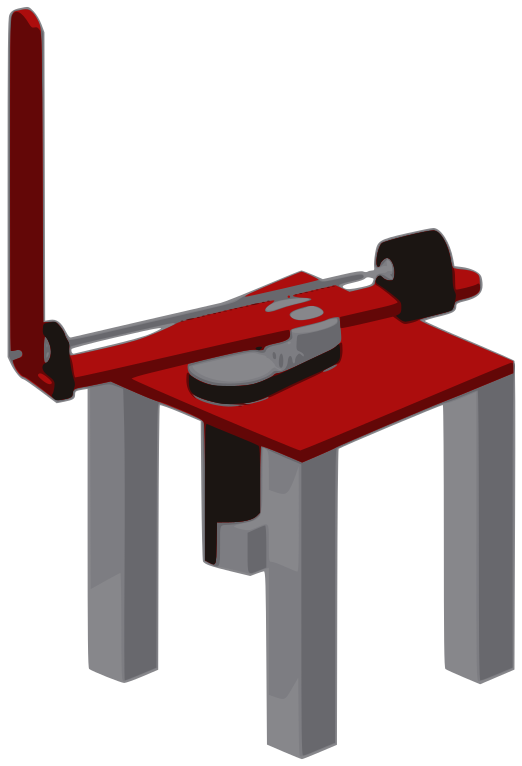
\includegraphics[height=12cm]{Title/Cover.png}\\[.5cm]
			% Title
			\HRule \\[0.4cm]
			{ \LARGE \bfseries Furuta Pendulum\\[0.2cm]}\small ASEN 5115 :: Mechatronics\\[0.4cm]
			\HRule \\[1cm]
			% Author and supervisor
				\begin{minipage}{0.4\textwidth}
					\begin{flushleft} \large
						\hspace*{-1em}\emph{Authors:}\\
						Zachary \textsc{Vogel}\\
					\end{flushleft}
				\end{minipage}
				\begin{minipage}{0.4\textwidth}
					\begin{flushright} \large
						\hspace{-2em}\emph{ } \\
						Maurice \textsc{Woods}
					\end{flushright}
				\end{minipage}
				\vfill
				\vspace{.75cm}
			% Bottom of the page
				\begin{minipage}{0.4\textwidth}
					\begin{flushleft} 
						
\includegraphics[width=2cm]{Title/CUSeal.jpg}\\
					\end{flushleft}
				\end{minipage}
				\begin{minipage}{0.4\textwidth}
					\begin{flushright}
						
\includegraphics[width=1.75cm]{Title/CULogo.jpg}\\
					\end{flushright}
				\end{minipage}\\
			{\small 2 May 2016}\\
		\end{center}
	\end{titlepage}
\newpage

%%%%%%%%%%%%%%%%%%%% PRE-DOCUMENT CONTENTS %%%%%%%%%%%%%%%%%%%%%%
%Table of Contents
\setcounter{tocdepth}{1}
\tableofcontents	
\newpage

%%%%%%%%%%%%%%%%%%%% FORMATTING NOTES %%%%%%%%%%%%%%%%%%%%%%
%%%%%%%%%%%%%%%% (Don't delete/uncomment) %%%%%%%%%%%%%%%%%%
%
%\begin{sect} %Custom environment for section
%\section{SECTION HEADING} %No content in sect environment
%\end{sect}
%   
%    SECTION CONTENT\\
%    \subsection{SUBSECTION HEADING}
%        SUBSECTION CONTENT\\
%        
%        \begin{subsubs} %Custom environment for subsubsection
%        \subsubsection{SUBSUBSECTION HEADING}
%            SUBSUBSECTION CONTENT\\
%        \end{subsubs}

%%%%%%%%%%%%%%%%%%%% DOCUMENT CONTENTS %%%%%%%%%%%%%%%%%%%%%%
\begin{sect} %Custom environment for section
\section{Introduction}
    The inverted pendulum is the staple of any controls-based engineering curriculum; by displacing a cart from which a pendulum hangs, one can easily derive a controller that will swing-up and balance the pendulum in the upright position. Here, we've explored a modified system, where the linearly-displaced cart is replaced by a rotating armature, from which hangs our pendulum. We will construct a benchtop model and design a custom controller to balance the pendulum based on its specific inertial characteristics.
\end{sect}

\begin{sect}
\section{Model}
    To begin, our research referenced a paper by mechanical engineering students in an Advanced System Dynamics and Control course at MIT titled "Furuta Pendulum", written in Fall 2013. In the paper, students characterized a futura pendulum of their own design and design a controller based of the mechanics they derive for the system. Following the model and general concepts of that team we designed and built our own system. We chose not to write down the values the equations that fill in the state equations, the group from MIT used symbolic variables in Matlab to find the solution.
    
\end{sect}


\begin{sect}
\section{Hardware and System Identification}%https://www.sharelatex.com/project/572acad43f0401db1320b9ae
    To begin, we were provided a collection of incomplete legacy hardware, used by a past team to construct a Furuta Pendulum. Ultimately, only the drive motor and the legs of the pendulum stand were reused as the remaining hardware was unusable. The revised pendulum eliminated the encoder cable by incorporating a slip ring, allowing the pendulum to spin without limit. Because the slip ring replaced the motor as the pendulum's pivot, the motor was displaced, requiring a timing belt/pulley assembly to transfer torque to the pendulum.\\
    %which was dope
    The pendulum's motion is controlled by a Teensy 3.2 microcontroller which senses the displacement of two rotary encoders (one that measures the rotation of the motor and one that measures the rotation of the pendulum rod), both quadrature. The Pittman brushed DC motor is controlled using a Pololu high power motor driver which is provided a PWM signal by the microcontroller. The motor is rated to 19V (however the motor controller is rated to 18V) and the remaining hardware is rated to 5V, so two power supplies are used to provide these two voltage levels to their respective components.\\
    
  %Mo talking about cad stuff
  In order to accurately calculate the inertial parameters used to apply the controller to our specific pendulum, we used Autodesk Inventor CAD software to determine the center of mass and moment of inertia for each arm of the Furuta pendulum. In doing so, we found the following parameters:
  \begin{table}[H]
      \centering
      \begin{tabular}{r l c r l}
          $m_1$=     & 0.107kg   & \qquad & $m_2$=        & 0.077kg \\
          $l_1$=    & 0.15m          & \qquad & $l_2$=        & 0.19m\\
          $c_{x1}$=  & 0.0m      & \qquad & $c_{2x}$=     & 0.125m\\
          $c_{y1}$=  & 0.0m      & \qquad & $c_{2y}$=     & 0.0m\\
          $c_{z1}$=  & 0.0m      & \qquad & $c_{2z}$=     & 0.0544m\\
                    &           & \qquad & $I_{2xx}$=    & 0.0003035 kg m$^2$ \\
                    &           & \qquad & $I_{2yy}$=    & 0.0005484 kg m$^2$ \\
          $I_{1zz}$= & 0.0005622 kg m$^2$ & \qquad & $I_{2zz}$= & 0.0002499 kg m$^2$\\
                    &           & \qquad & $I_{2xz}$=    & 0.000146 kg m$^2$\\
      \end{tabular}
      \caption{Parameters for our Furuta pendulum. The subscript $_1$ refers to the drive arm (left figure below) and the subscript $_2$ refers to the pendulum arm (right figure below). CoM distances are measured from the pivot point of the drive arm. Below, the coordinate frame and centers of mass are labeled.}
  \end{table}
  \begin{tabular}{c c}
    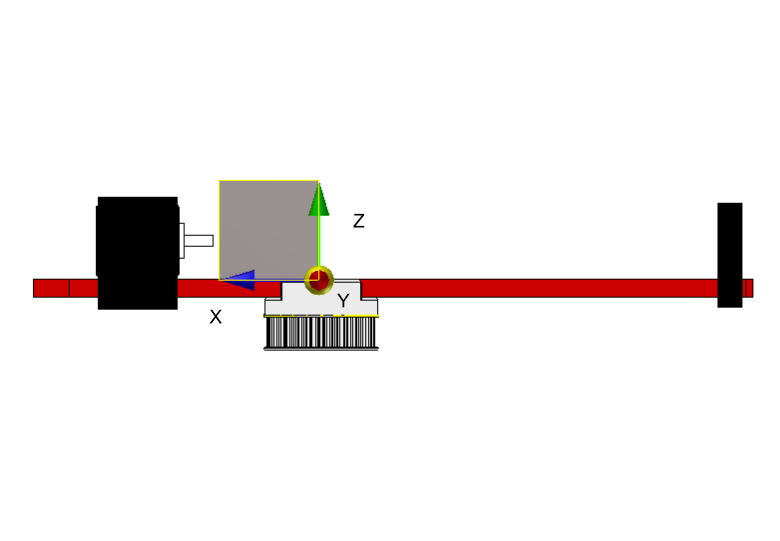
\includegraphics[width=3in]{Images/ArmMotor.png}   &     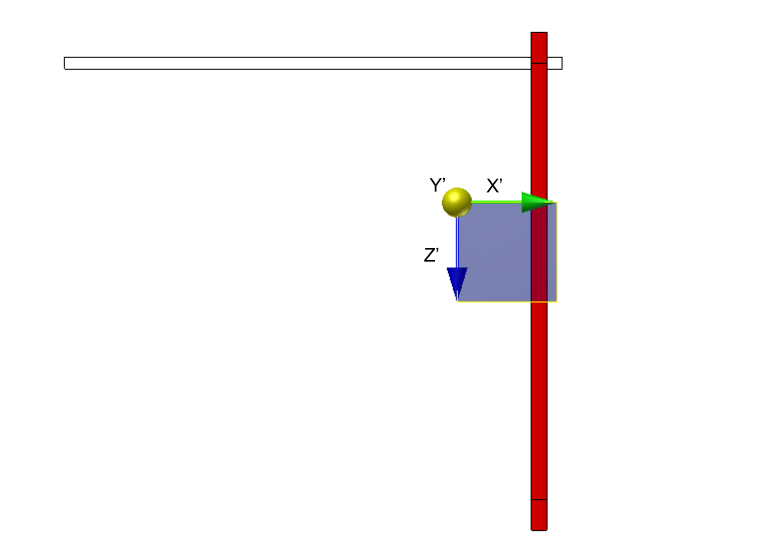
\includegraphics[width=3in]{Images/ArmPendulum.png}
  \end{tabular}
  
  
  
  To find the correct damping coefficient for the inverted pendulum rod, we needed to take data directly from the system. This was accomplished with some of the code in the Appendix. We utilized the prebuilt encoder library and the micros function call to find the rod position at a given time. Then we held the top rod still and gave it a tap. Print all that data nicely formatted over to Matlab, take the maximum and multiply by a few constants as seen in a section of the Matlab code, and you have the desired damping value.
    
    
    Refer to the Bill of Materials, linked in the Appendix for more information on the parts used and pictures of the hardware.
\end{sect}

\begin{sect}
\section{Analysis and Simulation}
Finally having identified all of our systems values, we needed to see what the response of our system looked like in simulation and design a controller or two from there. We took the state space equations directly from the "Furuta Pendulum" group at MIT[1]. Once calculated with our values and lack of a current sensor the state space equations became:
\[\begin{split}\begin{bmatrix}\theta_1\\\theta_2\\\dot{\theta_1}\\\dot{\theta_2}\\i\end{bmatrix}=\pmb{\dot{x}}=\begin{bmatrix}0 & 0 & 1 & 0 & 0\\0 & 0 &0 &1&0\\0&16.69&-1.079&-0.01476&9.729\\0&53.20&-0.7660&-0.07886&6.908\\0&0&-11.33&0&-1860\end{bmatrix}\begin{bmatrix}\theta_1\\\theta_2\\\dot{\theta_1}\\\dot{\theta_2}\\i\end{bmatrix}+\begin{bmatrix}0\\0\\0\\0\\666.6\end{bmatrix}\pmb{\mathcal{V}}\\\begin{bmatrix}\theta_1\\\theta_2\end{bmatrix}=\begin{bmatrix}1&0&0&0&0\\0&1&0&0&0\end{bmatrix}\pmb{x}+\begin{bmatrix}0\\0\end{bmatrix}\pmb{\mathcal{V}}\end{split}\]

Having recently been in Digital Control I, Zach, decided to design a fully digital controller. Thus I converted the system to discrete time with a sample rate that was 40 times the fastest pole frequency. That turned out to be $T=0.003500$sec at one point in the design process and we stuck with that for the rest of the project. With that decided the discrete time equations converted to modal form where:
\[\begin{split}\pmb{x}(kT+T)=F\pmb{x}(kT)+Gu(kT)=\begin{bmatrix}1&0&0&0&0\\0&1.025&0&0&0\\0&0&0.9742&0&0\\0&0&0&0.99692&0\\0&0&0&0&0.001489\end{bmatrix}\pmb{x}(kT)+\begin{bmatrix}0.0429\\0.03188\\-0.04185\\0.005669\\0.3581\end{bmatrix}u(kT)\\y(kT)=\begin{bmatrix}0.25&0.00468&0.005635&-0.1875&0.000002812\\0&0.0167&0.01591&0.002542&0.000001997\end{bmatrix}x(kT)+\pmb{0}u(kT)\end{split}\]

As can bee seen, the system has one marginally stable pole at 1 and one unstable pole at 1.025. Without any kind of feedback the step response of course just blow up. This can be seen in the root locus of the system as well. At this point we decided to move the poles arbitrarily to 0.99,0.998,0.95,0.97,0.0015 and the observer poles to -0.01, -0.05, 0.951, 0.97, 0.0. We ended up playing around with a bunch of values based on the Simulink results to no avail as regardless of if the simulation worked it still failed. Those are the values that gave the rest of the results in this section though.
\begin{figure}[H]
    \centering
    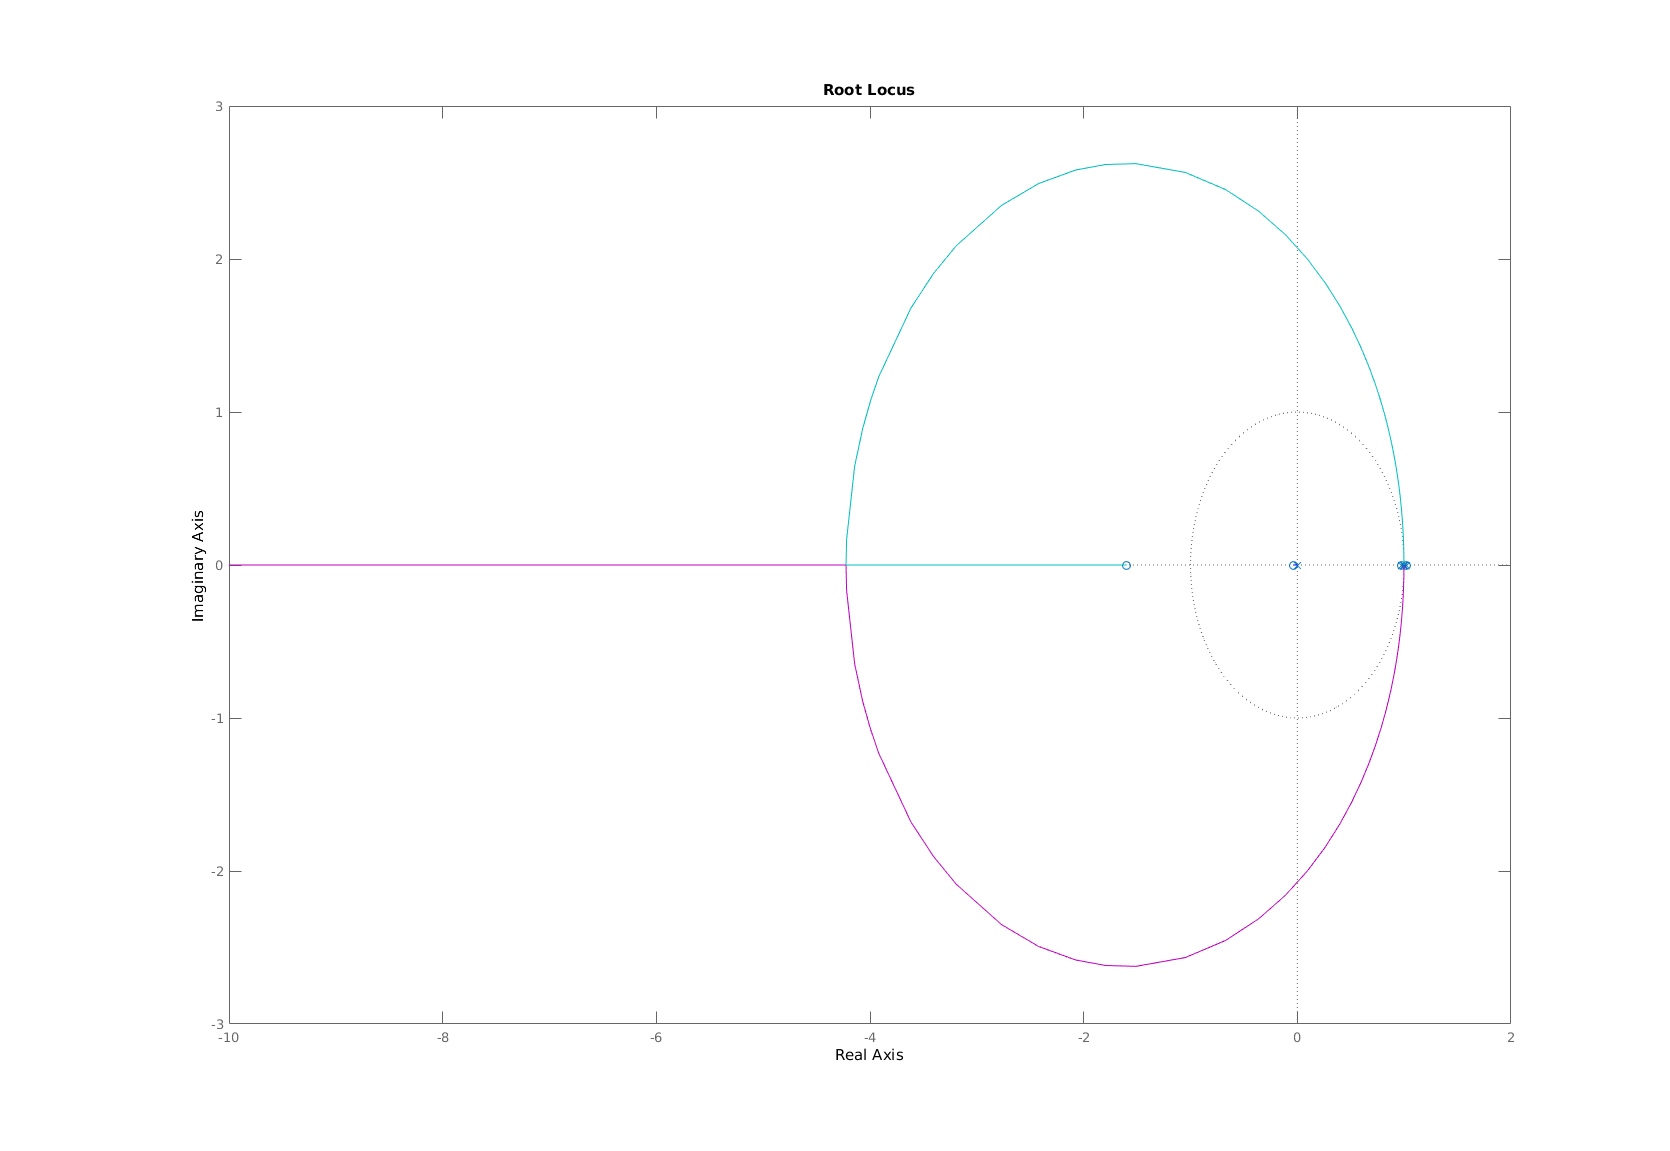
\includegraphics[width=0.8\textwidth]{Images/rlocus.png}
    \caption{Root Locus of the System}
\end{figure}
With the values finally set, we implemented a Simulink model with the following diagram taken from Lucy Pao's Digital Control class. The diagram can be seen below. As well as all of the corresponding plots. The response is generally what we wanted. Unfortunately that didn't translate later. The feed in matrices were calculated based on the reference effecting the motor, then the rod would stabilize.

\begin{figure}[H]
    \centering
    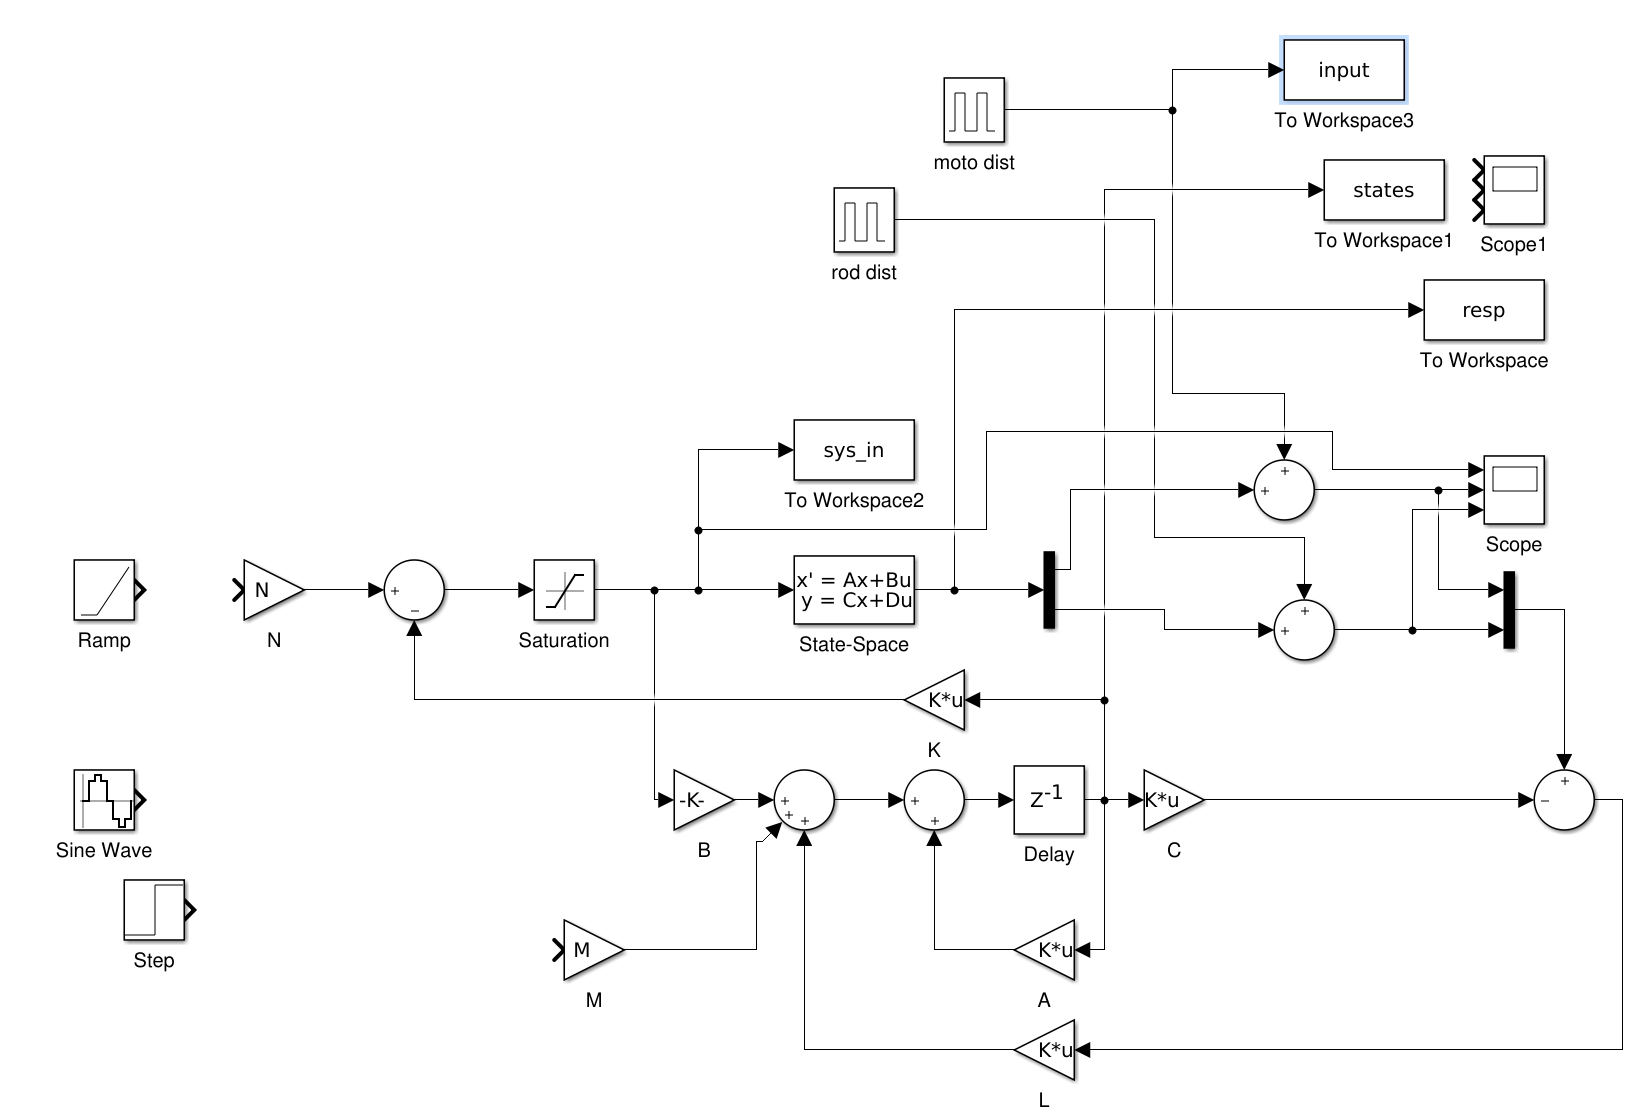
\includegraphics[width=0.8\textwidth]{Images/observer.png}
    \caption{Since}
\end{figure}
\begin{figure}[H]
    \centering
    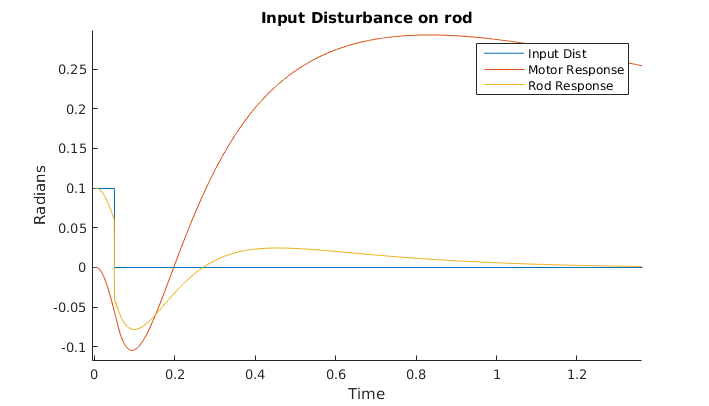
\includegraphics[width=0.8\textwidth]{Images/input_dist.png}
    \caption{As you can see, a light tap on the rod provides a cool response in sim.}
\end{figure}
\begin{figure}[H]
    \centering
    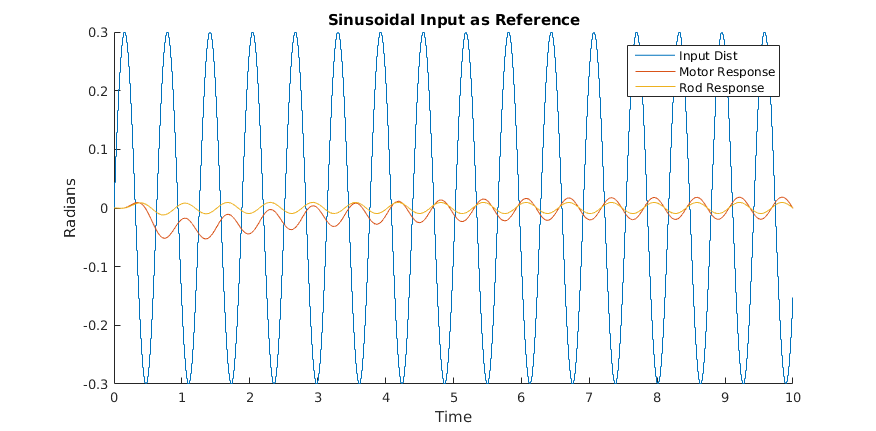
\includegraphics[width=0.8\textwidth]{Images/sin_in.png}
    \caption{Theoretically should have been able to make a cool oscillatory motion too.}
\end{figure}
\begin{figure}[H]
    \centering
    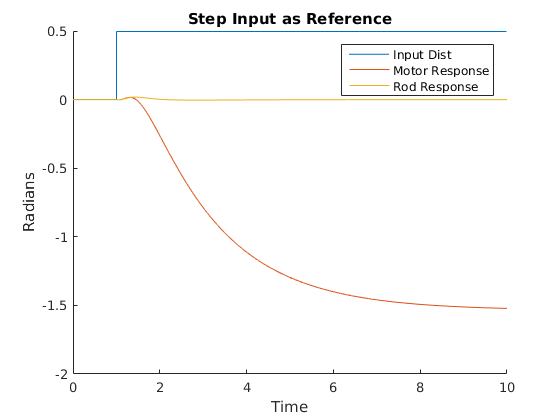
\includegraphics[width=0.8\textwidth]{Images/Step_in.png}
    \caption{Here we see the step response, which also manages to keep balance.}
\end{figure}
\begin{figure}[H]
    \centering
    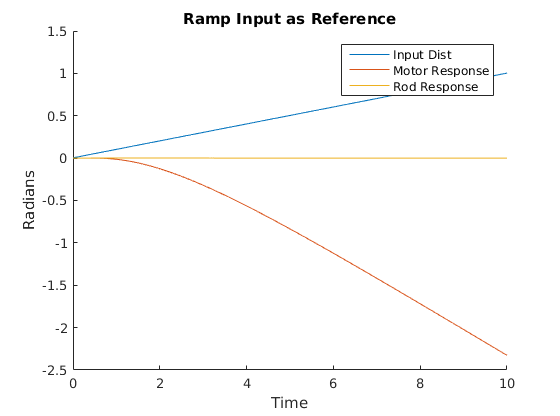
\includegraphics[width=0.8\textwidth]{Images/ramp_in.png}
    \caption{Finally the ramp input, which should keep it spinning slowly indefinitely.}
\end{figure}

Since the observer ended up not working, we designed a PID quickly using PID Tuner. The figure below shows its disturbance rejection. The values were K=98.936, Kd=6.6904, and Ki=348.9383. We just tuned this till it looked about right and those were the values we ended with. Certainly not a robust controller by any means.
\begin{figure}[H]
    \centering
    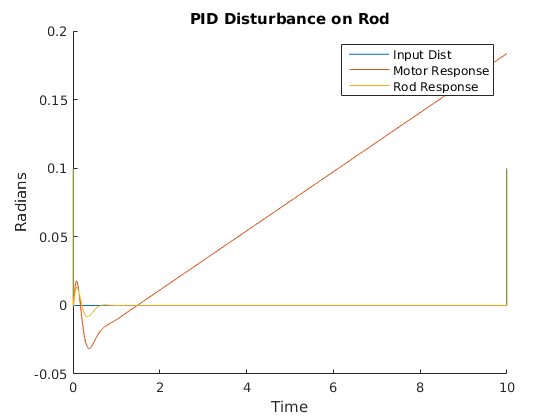
\includegraphics[width=0.8\textwidth]{Images/PID_DIST.png}
    \caption{The observer model in Simulink}
\end{figure}


\end{sect}


\begin{sect}
\section{Implementation}
The code mainly consists of two Real-Time Operating System Tasks. The first, which determines the two output states based on the encoder pulses and drives the motor. The second, which runs the controller that takes in the output states and outputs the encoder pulses. These are protected with binary Semaphores. The encoder pulses for both sets of encoders are kept track of by four interrupts implemented in the Teensy encoder library. Similarly, we use the timer library to implement an interrupt that tells us when to run our tasks. These tasks would be prevented from running by another set of binary semaphores, but that seemed to cause a hard fault on the microcontroller. This could be seen by the microcontroller moving to the Hard fault interrupt which is an infinite loop that blinks the LED.

The matrix math for the controller is done with two dimensional arrays and proper indexing. Most of the values are floats, but that is converted to an integer, so that it can be used with the PWM. The PWM pin that drives the motor has a 16 bit resolution up to 65535. Given our 18.1 volt motor that gives an easy conversion. The encoder outputs are similarly converted to radians using the ticks per cycle.
\end{sect}

\begin{sect}
\section{Results}
We began testing with the state observer. This didn't work at all either due to the instability in the growth of the states due to improper matrix multiplication, or instability in the controller. We know this because the floating point numbers defining the states in the c code blew up to the maximum floating point value relatively quickly. Could also be the modeling of the system dynamics or the system identification, specifically the damping coefficient. Since this wasn't working and Zach didn't really know how to go about fixing the observer design, that is where it ended for now. The PID controller kind of work and considering Zach implemented it Thursday morning it looked alright. This can be seen in the video that is inside the zip file with this report (link provided in the Appendix).
\end{sect}

\begin{sect}
\section{Final Thoughts and Further Work}
While the centerpiece of this project is the controller, which is responsible for making the pendulum an interesting and eye-catching demonstration piece, the assembly has the added benefit of being built from materials that are readily available, relatively inexpensive, and easily modified, making it ideal for an small academic research project. With more financial resources, the model could be improved to incorporate more sensors for monitoring the motion of the pendulum and the effects of the motor while also considering nonlinear effects. We would also be able to construct a more stable platform from aluminum to minimize vibrations and disturbances, and implement a better controller like a linear quadratic regulator or Kalman filter. Throughout the project we have applied knowledge learned from other classes to a problem and although the controller didn't work properly we were able to garnet a lot of experience from implementing the various parts of this project.

\end{sect}

\begin{sect}
\section{References}
\begin{enumerate}[ {[}1{]} ]

         \item Andrew Careaga Houck, Robert Kevin Katzschmann, Joao Luiz Almeida Souza Ramos. 
        "Furuta Pendulum". 
        Massachusetts Institute of Technology, Department of Mechanical Engineering, 2.151 Advanced System Dynamics \& Control, 2013.
    \end{enumerate}
\end{sect}

\newpage

\begin{sect}
\section{Appendix}
    \subsection{Links and Files}
    Here we provide links to a video of the performance of the pendulum, as well as a repository of the CAD models used to design and assemble the mechanical model.\\
    \begin{itemize}
        \item \href{https://drive.google.com/open?id=0BwfJh1j5fkByLVJjS1Q5cDhHUXM}{CAD Files}
        \item \href{https://goo.gl/photos/yyPnPPLxGd5WqKR46}{Demonstration Video}
    \end{itemize}
    \subsection{Matlab Code}
\lstset{language=Matlab,%
    %basicstyle=\color{red},
    breaklines=true,%
    morekeywords={matlab2tikz},
    keywordstyle=\color{blue},%
    morekeywords=[2]{1}, keywordstyle=[2]{\color{black}},
    identifierstyle=\color{black},%
    stringstyle=\color{magenta},
    commentstyle=\color{green},%
    showstringspaces=false,%without this there will be a symbol in the places where there is a space
    numbers=left,%
    numberstyle={\tiny \color{black}},% size of the numbers
    numbersep=9pt, % this defines how far the numbers are from the text
    emph=[1]{for,end,break},emphstyle=[1]\color{red}, %some words to emphasise
    %emph=[2]{word1,word2}, emphstyle=[2]{style},    
}
\begin{lstlisting}
%Zachary Vogel
%Real design of Control

%be clear that the first state is the motor angle
%second is the rod angle
%third and 4th are their derivatives
%fifth is motor current


%actual known values
g=9.8;%m/s^2 gravity
Rm=2.79; %ohms terminal resistance
kt=0.017; %Nm/A torque constant
Lm=.0015; %milli Henries, motor inductance
Jm=1.62*10^(-6); %kgm^2 motor inertia

%values from paper, need to find these before actual implementation

m1=0.107;%mass of first rod?
m2=0.077;%mass of second rod?
L1=0.125;%length from motor shaft to center of mass of motor rod+inverted pendulum rod
l1=0.0;%length from motor shaft to Center of mass of motor rod
L2=0.195;%length of inverted pendulum rod
l2=0.0544;%length from plane of motor rod to center of mass of motor rod+inverrted pendulum
%b1=6.0*10^(-4);%damping 1
b1=6.0*10^(-4)*pi;%viscous damping is 1.34*10^(-6)*pi
%b2=0.000109468513065094;%damping 2 from system id
b2=3.63316395*10^(-5);
%Inertia tensors are a 3 element vector of torques in 3 rotational
%directions equal to a 3X3 matrix of inertias times a 3 element vector of
%angular accelerations.

I1z=0.00056216; %Izz Inertia only one from 
I2x=0.0003035; %other inertias, measured in CAD
I2y=0.0005484;
I2z=0.0002499;
I2xz=0.0001463;

den=(I2x*I1z-I2xz^2+I2x*I2z+I2x*L1^2*m2+I2x*l1^2*m1+I1z*l2^2*m2+I2z*l2^2*m2+2*I2xz*L1*l2*m2+l1^2*l2^2*m1*m2);

A11=0;
A12=-(g*l2*m2*(I2xz-L1*l2*m2))/den;
A13=-(b1*(m2*l2^2+I2x))/den;
A14=(b2*(I2xz-L1*l2*m2))/den;
A15=(kt*(m2*l2^2+I2x))/den;

A21=0;
A22=(g*l2*m2*(m2*L1^2+m1*l1^2+I1z*I2z))/den;
A23=(b1*(I2xz-L1*l2*m2))/den;
A24=-(b2*(m2*L1^2+m1*l1^2+I1z+I2z))/den;
A25=-(kt*(I2xz-L1*l2*m2))/den;

A31=0;
A32=0;
A33=-kt/Lm;
A34=0;
A35=-Rm/Lm;

B1=0;
B2=0;
B3=1/Lm;

A=[0 0 1 0 0;0 0 0 1 0;A11 A12 A13 A14 A15;A21 A22 A23 A24 A25;A31 A32 A33 A34 A35];
B=[0;0;B1;B2;B3];
C=[1 0 0 0 0;0 1 0 0 0];
D=[0;0];

sys1=ss(A,B,C,D);
[Wn,zeta]=damp(sys1);
rank(obsv(A,C));
wn=min(Wn(Wn>0));
Ts=wn/(40*pi);
Ts=0.0035;
sys=c2d(sys1,Ts);
%pzmap(sys)
K=place(sys.a,sys.b,[0.99 0.998 0.95 0.97 0.0015])
L=place(sys.a',sys.c',[-0.01 -0.05 0.951 0.97 0.0])'

NMAT=[sys.a-diag([1,1,1,1,1]), sys.b;sys.c(1,:),[0]];

NMAT=inv(NMAT);

r=NMAT*[0;0;0;0;0;1];
N=r(6)+K*r(1:5);
M=sys.b*N;


%observer poles
F2=sys.a-sys.b*K-L(:,2)*sys.c(2,:);
G2=L(:,2);
H2=K;
J2=0;
[num1,den1]=ss2tf(F2,G2,H2,J2);
[num2,den2]=tf2zp(num1,den1);


F1=sys.a-sys.b*K-L(:,1)*sys.c(1,:);
G1=L(:,1);
H1=K;
J1=0;
[num3,den3]=ss2tf(F1,G1,H1,J1);
[num4,den4]=tf2zp(num3,den3);

A1=A;
B1=B;
C1=[0 1 0 0 0];
%C1=C;
%D1=D;
D1=0;
sys4=ss(A1,B1,C1,D1);
sysd=c2d(sys4,Ts);
sysm=canon(sysd,'modal');
sysc=canon(sysd,'companion');
K1=place(sysc.a,sysc.b,[0,0.1,0.95,0.98,0.2]);
L1=place(sysc.a,sysc.c',[0,0.05,0.95,0.96,0.1])';


PIDK=98.936;
PIDKD=6.6904;
PIDKI=348.9383;
\end{lstlisting}

    \subsection{MicroController Code}
    \lstdefinestyle{customc}{
  belowcaptionskip=1\baselineskip,
  breaklines=true,
  frame=L,
  xleftmargin=\parindent,
  language=C,
  showstringspaces=false,
  basicstyle=\footnotesize\ttfamily,
  keywordstyle=\bfseries\color{green},
  commentstyle=\itshape\color{purple},
  identifierstyle=\color{blue},
  stringstyle=\color{orange},
}

\lstset{escapechar=@,style=customc}
    The code we used to identify the damping factor of the encoder based on the motor.
\begin{lstlisting}
#include <Encoder.h>


Encoder knobLeft(5, 6);
Encoder knobRight(7, 8);


long a=0;

void setup() {
  Serial.begin(9600);
  Serial.println("TwoKnobs Encoder Test:");
  a=micros();
}

long positionLeft  = -999;
long positionRight = -999;


void loop() {
  long newLeft, newRight;
  newLeft = knobLeft.read();
  newRight = knobRight.read();
  if (newLeft != positionLeft || newRight != positionRight) {
    
    //Serial.print("Left = ");
    Serial.print(newLeft);
    Serial.print(",");
    Serial.print(micros()-a);
    Serial.print(";");
    Serial.println();

    positionLeft = newLeft;
    positionRight = newRight;
    
  }

  // if a character is sent from the serial monitor,
  // reset both back to zero.
  if (Serial.available()) {
    Serial.read();
    Serial.println("Reset both knobs to zero");
    knobLeft.write(0);
    knobRight.write(0);
  }
}
\end{lstlisting}
The final code for the state observer with state feedback
\begin{lstlisting}
#include <FreeRTOS_ARM.h>
#include <Encoder.h>

//#define ENCODER_USE_INTERRUPTS 1
//#define SUPDOG 1


#define MOTOPWM 9
#define MOTODIR 10
#define MOTOENCL 3
#define MOTOENCR 4
#define RODENCL 5
#define RODENCR 6

const float A[5][5]={{1.0, 0.0,     0.0,         0.0,       0.0},
                    {0.0, 1.025,    0.0,         0.0,       0.0},
                    {0.0, 0.0,      0.9742,      0.0,       0.0},
                    {0.0, 0.0,    0.0,         0.9969,    0.0},
                    {0.0, 0.0,      0.0,         0.0,       0.001489}};
const float B[]={0.0429,
                 0.03188,
                 -0.04185,
                 0.05669,
                 0.3581};
const float C[2][5]={{0.25,0.00468,0.005635,-0.1874,0.000002812},
                      {0.0, 0.0167,0.01591,0.002542,0.000001997}};

const float L[5][2]={{1.055597,     -0.0018567},
                    {-0.00818119,      1.08129},
                    {12.875,   -0.4049},
                    {-2.08169,      9.38346},
                    {-3.3927 , -13.125}};
                    
const float K[]={-1.389,105.456,-3.502506,15.021901,0.03726};


SemaphoreHandle_t sem1,sem2;
volatile int run1=0,run2=0;

//built in encoder interrupts
Encoder MotoEnc(MOTOENCL,MOTOENCR);
Encoder rodEnc(RODENCL,RODENCR);

//built in timer interrupt
IntervalTimer sampletimer;

//onl shared variables
volatile float ymeas[2]={0.0,0.0};
volatile int unew=0;


void TimeSemEnable(void)
{
  //cause giving semaphores throws a fault
   run1++;
  run2++;
}



void Observer(void * params)
{
    float x[]={0.0,0.0,0.0,0.0,0.0};
    float xnew[5]={0.0,0.0,0.0,0.0,0.0};
    float utemp=0.0;
    int utempi=0;
    float yest[2]={0.0,0.0};
    float yerr[2]={0.0,0.0};
    float temp[5];
    int i;

#ifdef SUPDOG
    int time1=0;
    int maxtime=0;
#endif

    //Serial.println("do I get here");
    while(1)
    {
#ifdef SUPDOG
     time1=micros();
#endif
        while(run2==0);

        run2=0;

        

        utemp=0;
        yest[0]=0;
        yest[1]=0;




        //new state, output state
        for(i=0;i<5;i++)
        {
          x[i]=xnew[i];
          utemp+=K[i]*x[i];
          yest[0]+=C[0][i]*x[i];
          yest[1]+=C[1][i]*x[i];
        }

        /*Serial.print(yest[0]);
        Serial.print(",");
        Serial.println(yest[1]);*/
        
        //mutex_lock
        if(utemp>18)
        {
          utemp=18;
        }
        if(utemp <-18)
        {
          utemp=-18;
        }
        //Serial.println(utemp,8);
        utempi=(int)(utemp*65535.0/18.0);
/*#ifdef PRINTING*/
        Serial.print(x[0]);
        Serial.print(",");
        Serial.print(x[1]);
        Serial.print(",");
        Serial.print(x[2]);
        Serial.print(",");
        Serial.print(x[3]);
        Serial.print(",");
        Serial.println(x[4]);
/*#endif*/
        if(utempi>65535)
        {
          utempi=65535;
        }
        if(utempi<-65535)
        {
          utempi=-65535;
        }
 
        xSemaphoreTake(sem1,0);
        unew=utempi;
        xSemaphoreGive(sem1);
        //mutex unlock

        //mutex_lock
        xSemaphoreTake(sem2,0);
        yerr[0]=ymeas[0]-yest[0];
        yerr[1]=ymeas[1]-yest[1];
        //mutex unlock
        xSemaphoreGive(sem2);


        



        for(i=0;i<5;i++)
        {
          temp[i]=utemp*B[i]+yerr[0]*L[i][0]+yerr[1]*L[i][1];

        }
        for(i=0;i<5;i++)
        {
            xnew[i]=temp[i]+x[0]*A[i][0]+x[1]*A[i][1]+x[2]*A[i][2]+x[3]*A[i][3]+x[4]*A[i][4];
        }
        

/*#ifdef SUPDOG
        time1=micros()-time1;
        if(time1>maxtime)
        {
          maxtime=time1;
          //Serial.print("Observer max time was");
          //Serial.println(maxtime);
        }
#endif*/

        
    }
    //Serial.print("max time after 100000 trialswas");
    //Serial.print(maxtime);
    //Serial.println(" in microseconds");
    while(1);
}



void writer(void * params)
{

    double ytemp[2]={0.0,0.0};
    int utemp=0;

#ifdef SUPDOG
    int time1=0;
    int maxtime=0;
#endif




    sampletimer.priority(200);
    sampletimer.begin(TimeSemEnable,3500);
    //sampletimer.end();
    while(1)
    {

#ifdef SUPDOG
     time1=micros();
#endif  

        //mutex_lock
        while(run1==0)
        {
          vTaskDelay(1);
        }
        run1=0;

        ytemp[0]=0;
        ytemp[1]=0;

        ytemp[0]=(float)MotoEnc.read()*0.00349065850398868;
        ytemp[1]=(float)rodEnc.read()*0.00785398163397448;
        //Serial.println(ytemp[0]);
        //Serial.println(ytemp[1]);
        //mutex_lock
        xSemaphoreTake(sem2,0);
        ymeas[0]=ytemp[0];
        ymeas[1]=ytemp[1];
        xSemaphoreGive(sem2);
        //mutex unlock

        if(ytemp[1]>0.34||ytemp[1]<-0.34)
        {
          analogWrite(MOTOPWM,0);
        }
        else{
          xSemaphoreTake(sem1,0);
          utemp=unew;
          xSemaphoreGive(sem1);
        
          if(utemp<0)
          {
            utemp=-utemp;
            digitalWrite(MOTODIR,LOW);
          }
          else
          {
            digitalWrite(MOTODIR,HIGH);
          }
          analogWrite(MOTOPWM,utemp);
          //Serial.println(utemp);
        }
        //mutex unlock

        
        

        //xSemaphoreGive(run2);
        
#ifdef SUPDOG
        time1=micros()-time1;
        if(time1>maxtime)
        {
          maxtime=time1;
          //Serial.print("writer max time was");
          //Serial.println(maxtime);
        }
#endif
//Serial.println(time1);

        

    }
    //Serial.print("max time after 100000 trialswas");
    //Serial.print(oldtime);
    //Serial.println(" in microseconds");
    while(1);
}



void setup() {
    analogWriteFrequency(MOTOPWM,732.4218);
    analogWriteResolution(16);
    portBASE_TYPE s;
    pinMode(MOTODIR,OUTPUT);
    MotoEnc.write(0);
    rodEnc.write(0);
    s = xTaskCreate(Observer, NULL, 200, NULL, 3, NULL);
    s = xTaskCreate(writer,NULL,200,NULL,4,NULL);
    sem1=xSemaphoreCreateMutex();
    sem2=xSemaphoreCreateMutex();


//#ifdef TESTING
    Serial.begin(9600);
//#endif
  // start tasks
  vTaskStartScheduler();
  //Serial.println("Scheduler failed");
  while(1);
}
//------------------------------------------------------------------------------
// WARNING idle loop has a very small stack (configMINIMAL_STACK_SIZE)
// loop must never block
void loop() {
  // not used
}

\end{lstlisting}
The PID controller code
\begin{lstlisting}
const float PIDK=98.936;
const float PIDKD=6.6904;
const float PIDKI=348.9383;

const float DT=0.0035;

void PID(void * params)
{
    float pre_yerr=0.0;
    float integral=0.0;
    float derivative=0.0;
    float utemp=0.0;
    int utempi=0.0;

    float yerr=0.0;

    int i;

#ifdef SUPDOG
    int time1=0;
    int maxtime=0;
#endif

    //Serial.println("do I get here");
    while(1)
    {
#ifdef SUPDOG
     time1=micros();
#endif
        while(run2==0);

        run2=0;

        

        utemp=0;
        //calculate input

        if((yerr<0.01)||(yerr>0.01))
        {
          integral=integral+yerr*DT;
        }
        derivative=(yerr-pre_yerr)/DT;
        
        utemp=PIDK*yerr+PIDKI*integral+PIDKD*derivative;

        utempi=(int)(utemp*65535.0/18);
/*#ifdef PRINTING*/

/*#endif*/
        if(utempi>65535)
        {
          utempi=65535;
        }
        if(utempi<-65535)
        {
          utempi=-65535;
        }
 
        xSemaphoreTake(sem1,0);
        unew=utempi;
        xSemaphoreGive(sem1);
        //mutex unlock

        //mutex_lock
        xSemaphoreTake(sem2,0);
        yerr=ymeas[1];
        //mutex unlock
        xSemaphoreGive(sem2);
        yerr=-yerr;

        
    }
    //Serial.print("max time after 100000 trialswas");
    //Serial.print(maxtime);
    //Serial.println(" in microseconds");
    while(1);
}


\end{lstlisting}
    \subsection{Hardware}
        
        \begin{figure}[H]
            \centering
            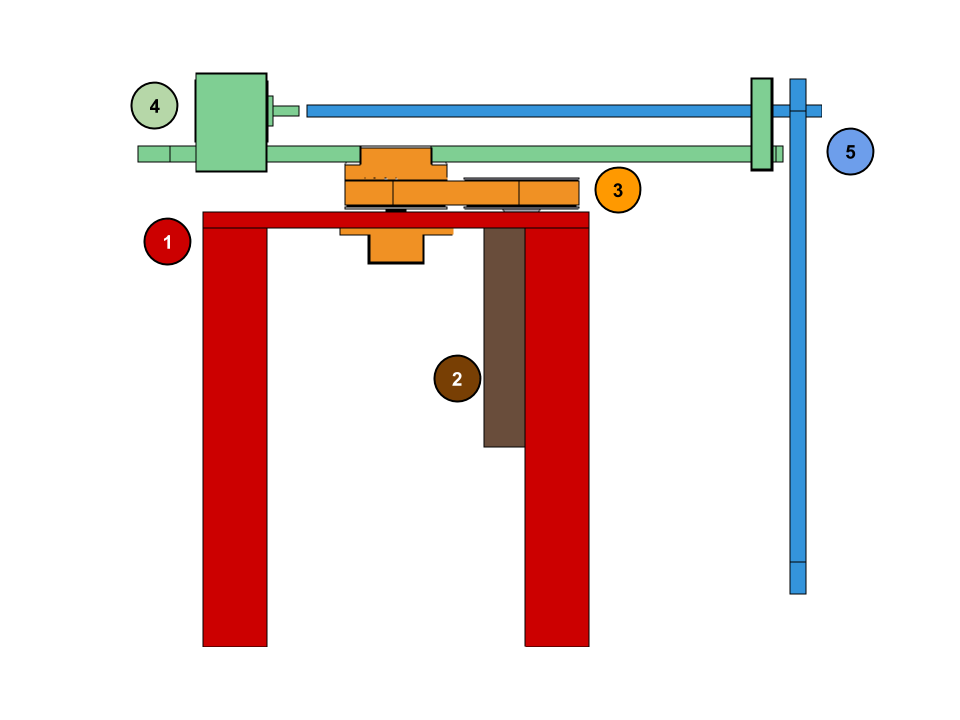
\includegraphics[width=5in]{Images/Assembly.png}
            \caption{A labeled model of the Furuta pendulum 1) 6" tall base stand 2) Motor and encoder 3) Timing belt transmission and slip ring 4) Drive arm and encoder 5) Pendulum arm}
            \label{fig:assembly}
        \end{figure}
        \begin{figure}[H]
            \centering
            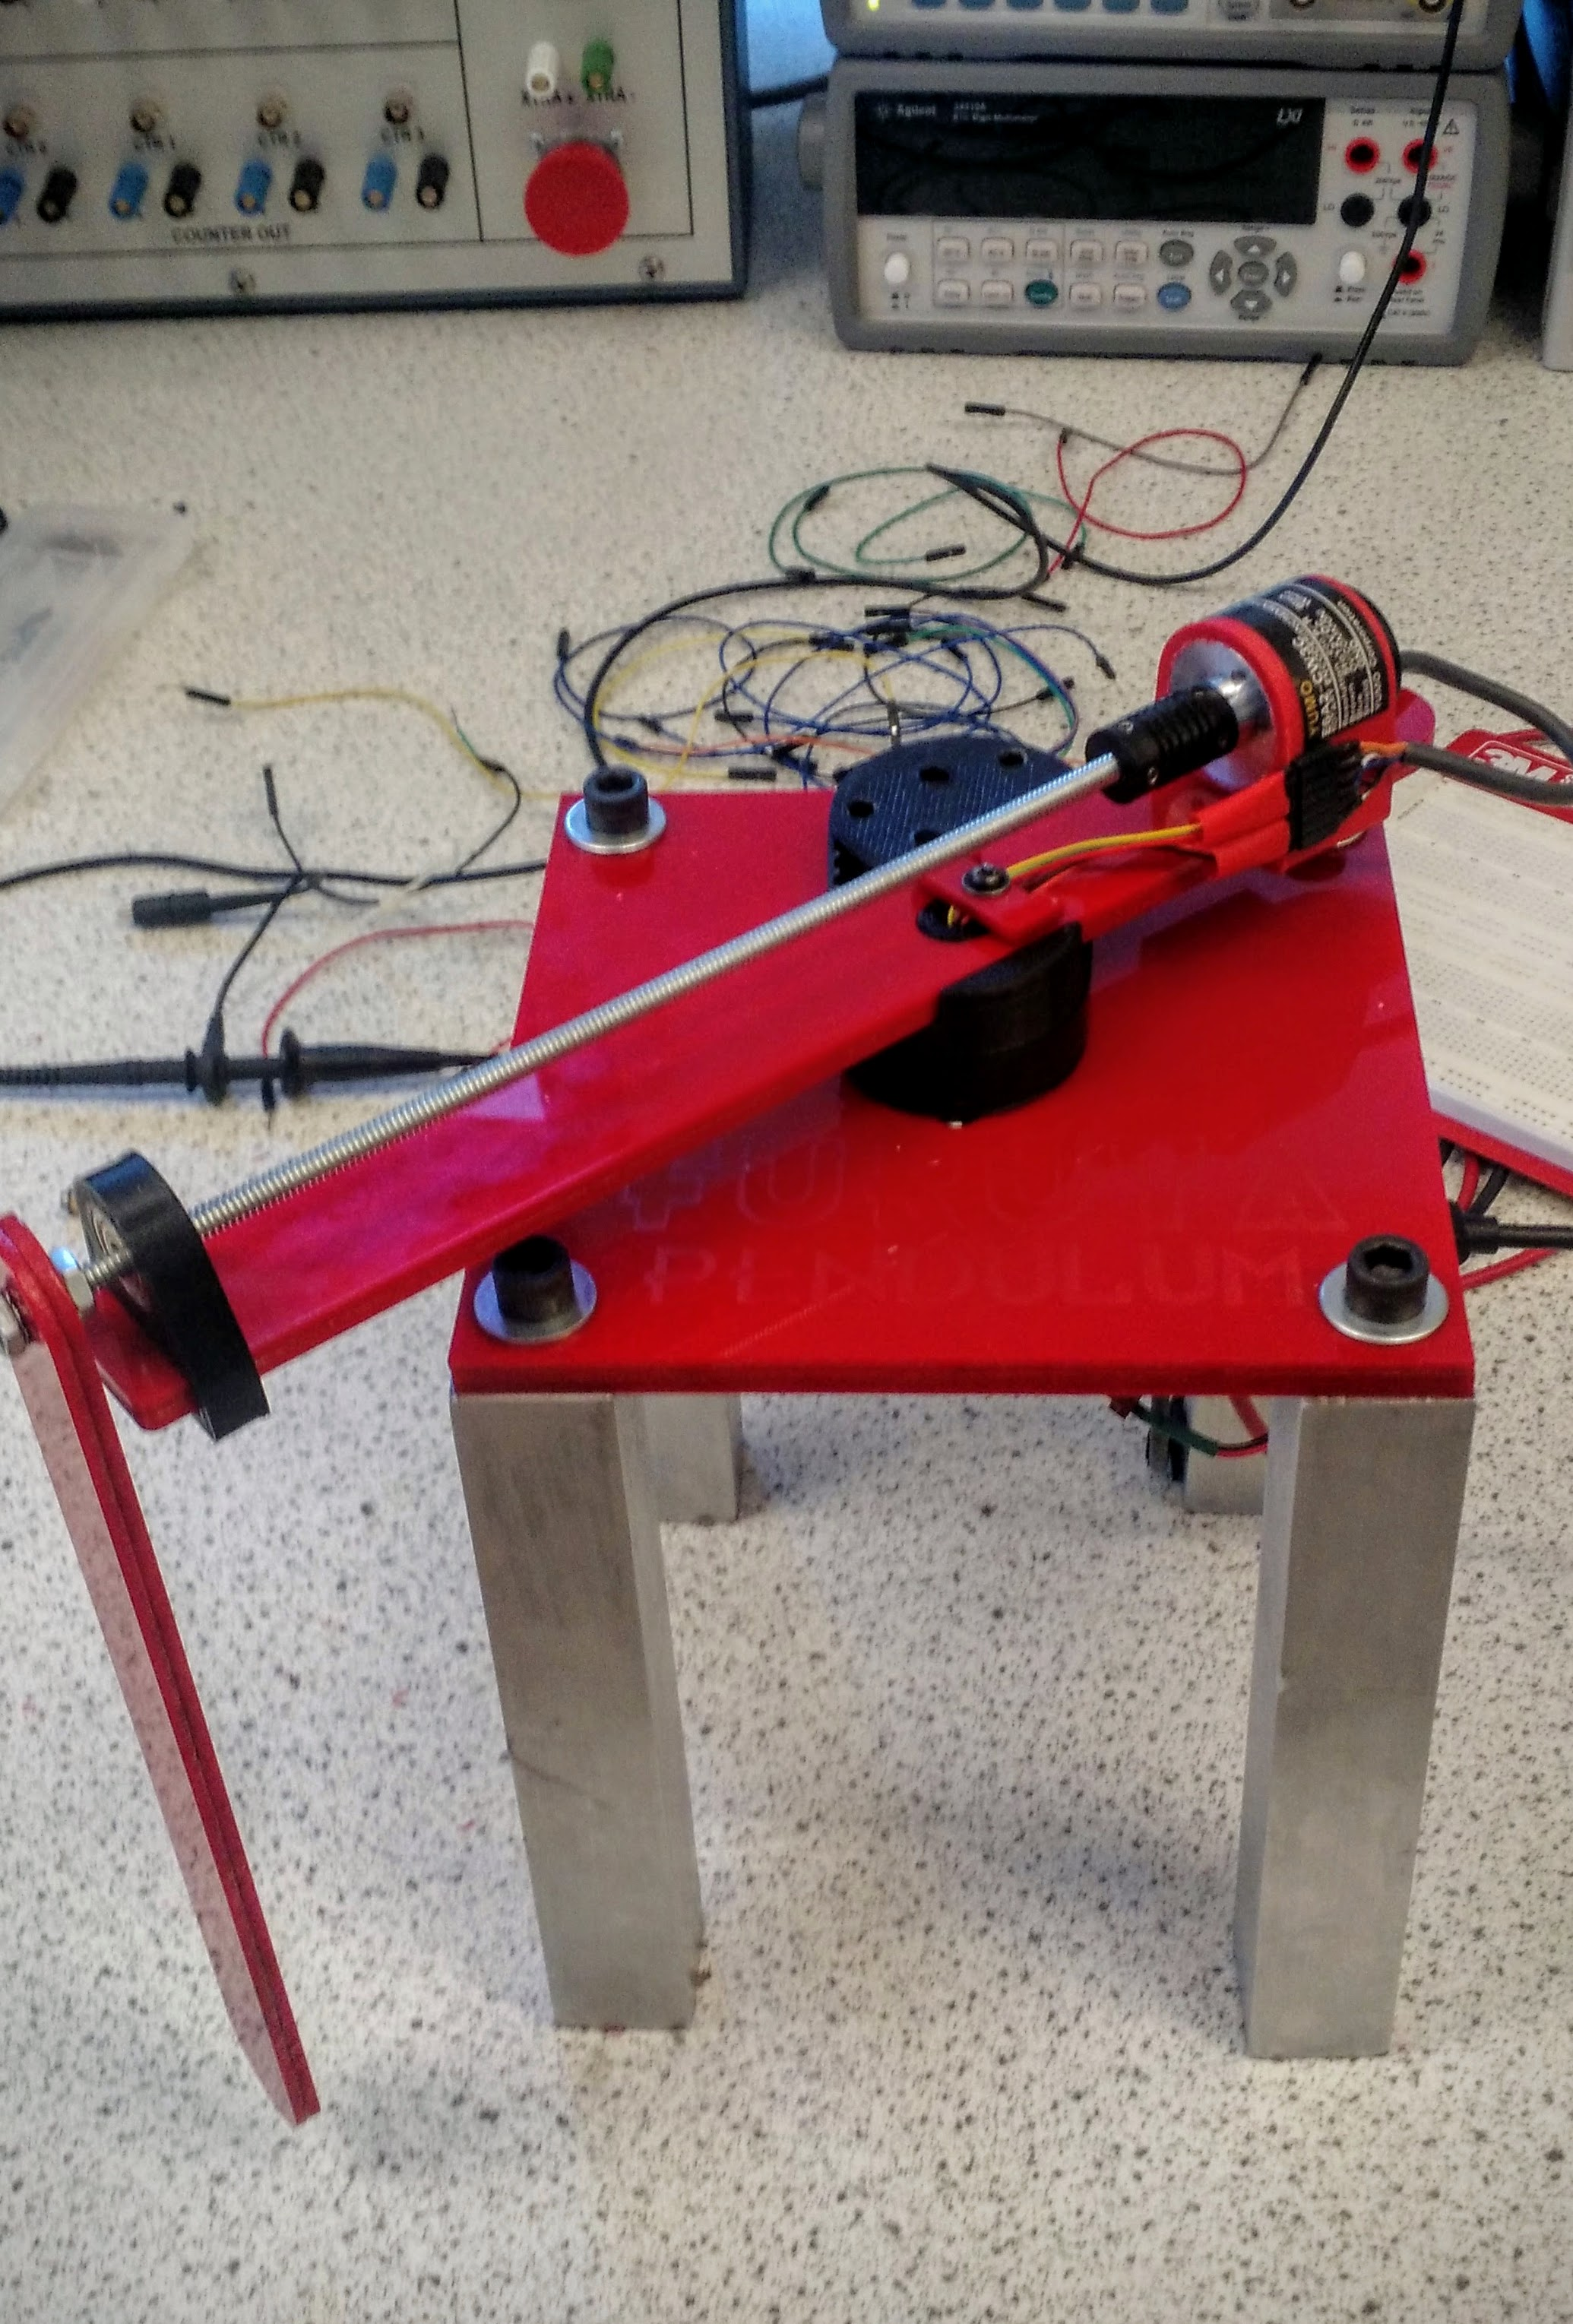
\includegraphics[width=4in]{Images/Bench.jpg}
            \caption{The fully assembled Furuta pendulum on the lab bench}
            \label{fig:bench}
        \end{figure}

\end{sect}



\end{document}
